\documentclass[a4paper, 12pt]{article}

\usepackage[no-math]{fontspec-xetex}
\setmainfont{CMU Sans Serif}
\usepackage[english, russian]{babel}

\usepackage{blindtext}
\usepackage{microtype}
\usepackage{geometry}

\usepackage{amsmath,amsfonts,amssymb,amsthm,mathtools}
\usepackage{MnSymbol}
\usepackage{physics}

\usepackage{graphicx, wrapfig, caption, subcaption}
\usepackage{color,xcolor}

\graphicspath{{figures/}}
\geometry{margin = 2 cm}
\geometry{bottom = 3 cm}

\title{Теор модель}
\author{Николай Грузинов}
\date{}%собрано \today}

\begin{document}
\maketitle

Вначале шарик падает с какой-то скоростью.
Как мы убедились, эта скорость больше той, которая должна установится, поэтому скорость будет постепенно замедлятся.
Можно считать, что под конец скорость уже установилась.

Из наших данных $x(t)$ можно извлечь установившуюся скорость $V$, вычислив угловой коэффициент прямой, проходящей через последние точки:
\begin{center}
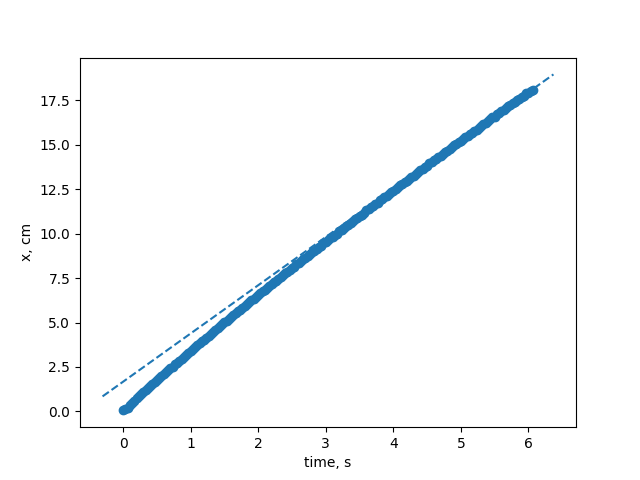
\includegraphics[width=0.7\linewidth]{approximation_0.png}
\end{center}

По $V$ можно найти вязкость $\eta$.
Возьму уравнение из методички, и немного перепишу.
Пусть $d$ --- диаметр шарика.
\[ m g = 3 \pi d \eta V+\rho g \frac{\pi d^{3}}{6} \]
\[ \eta = \frac{m g-\rho g \frac{\pi d^{3}}{6} }{3 \pi d V} \]

\section*{Как стоило бы делать, если бы не большая погрешность при численном дифференцировании?}

Пусть диаметр шарика $d$, масса $m$, плотность глицерина $\rho$, вязкость $\eta$.
Второй закон Ньютона для шарика, в проекции на ось OX, направленную вниз ($v_x > 0$)
% $\dv{v}{t} < 0$
\[ m \dv{v_x}{t} = -3 \pi \eta d v_x - \rho g \frac{\pi d^3}6 + mg \]
\[ \dv{v_x}{t} = -\frac{3 \pi \eta d}m v_x - \frac{\rho g \pi d^3}{6 m} + g \]
\[ \dv{v_x}{t} = -\frac{3 \pi \eta d}m \left(v_x + \frac{\frac{\rho g \pi d^3}{6} - mg}{3 \pi \eta d}\right) \]
Обозначу $c = \frac{mg - \frac{\rho g \pi d^3}{6}}{3 \pi \eta d}$ (установившаяся скорость), $v_x' = v_x - c$, $k = \frac{3 \pi \eta d}m$ (коэффициент в экспоненте).
Тогда $c > 0$, $k > 0$, и
\[ \dv{v_x'}{t} = -k v_x' \qquad\implies\qquad v_x'(t) = \bigl(v_{x_0} - c\bigr)\exp(-kt) \]
\[ v_x(t) = \bigl(v_{x_0} -  c\bigr)\exp(-kt) + c .\] 
\[
x(t) = \int_{0}^t v_x(t') \dd t' = \int_{0}^t \Bigl((v_{x_0} -  c)\exp(-kt') + c\Bigr) \dd t' =
	   \frac{(v_{x_0} -  c)}{-k}\exp(-kt') + ct + x_0
\]
Видно, что из $x(t)$ вытащить $k$ (и затем из $k$ выразить $\eta$) будет трудно, потребуется анализировать нелинейную регрессию.
Поэтому я предлагаю численно продифференцировать исходные данные $x(t)$, получить оттуда $v_x(t)$.
Это упростит задачу следующим образом.
Если считать, что в конце пути скорость установилась, то $c$ --- среднее из нескольких последних точек $v_x(t)$.
Тогда можно линеаризовать $v(t)$ следующим образом:
\[ \ln( v_x(t) - c ) = \ln(v_{x_0} -  c) - k t .\] 
Угловой коэффициент графика будет равен $-k$.

Чтобы получить $c$ более точно, можно попробовать поподбирать такие значения, при которых прологарифмированная зависимость будет лучше ложиться на прямую.
Из $c$ можно получить плотность глицерина $\rho$ и сравнить ее с табличными значениями.

При взгляде на данные видно, что ничего хорошего из этой идеи не выйдет, потому что качественно посчитать скорость в каждой точке не представляется возможным.
(Возможно, стоило попробовать это сгладить, используя moving average).
\begin{center}
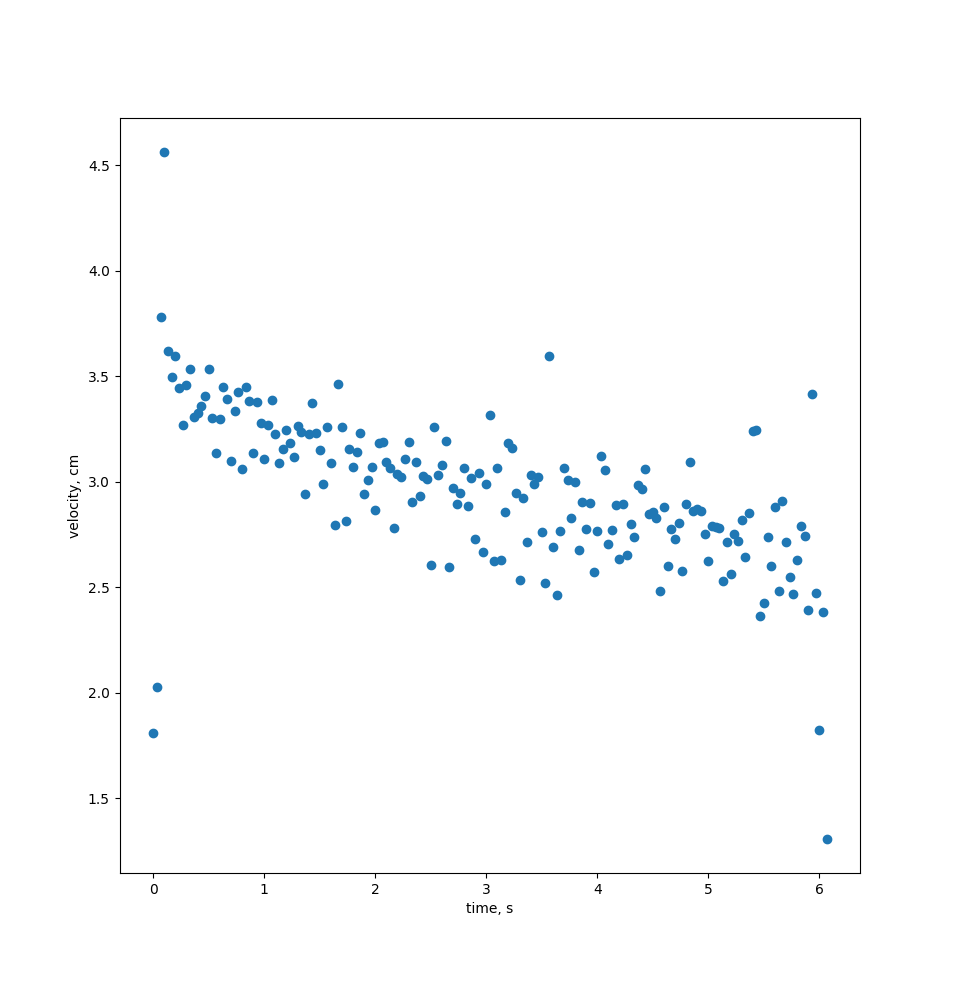
\includegraphics[width=0.6\linewidth]{bad_numericall_differentiation.png}
\end{center}

\section*{Как быстро устанавливается скорость шарика?}
Скорость задаётся уравнением
\[ v_x(t) = \bigl(v_{x_0} -  c\bigr)\exp(-kt) + c .\] 
Взяв какие-то разумные значения параметров, можно найти момент времени $\tau$ в который скорость будет отличаться, скажем, на $0.01$ от установившейся, то есть $v_x(\tau) = 1.01 c$:
\[ t = \frac{1}{k} \ln(\frac{v_{x_0} -  c}{v_x -  c}) .\]
\[ \tau = \frac{1}{k} \ln(\frac{v_{x_0} -  c}{0.01c}) .\]
Предположим, что мы отпустили шарик на высоте $h = 0.05$~м (на самом деле меньше).
Тогда $v_{x_0} = \sqrt{2gh} \approx 1$ м/с.
Для самого тяжелого шарика, примерно
\[ m = 3.9 \cdot 10^{-4} \text{ кг} \qquad d = 4 \cdot 10^{-3} \text{ м} .\]
Если взять табличное значение плотности $\rho = 1.12$~кг/м$^3$ и ожидаемое $\eta = 1.2$ для вязкости, то по вычислениям в файле $\verb|calculate_when_stable.py|$ получается
\[ c = 8.5 \text{ см/с} \qquad k = 116 \text{ 1/с} \qquad \tau = 0.06 \text{ c} .\]
А это означает, что шарик к моменту попадания в кадр уже имеет установившуюся скорость, и дальнейшее уменьшение скорости стоит объяснять изменением вязкости.
Тогда можно считать, что в каждый момент времени скорость --- установившаяся для данной глубины, а данные обработать следующим образом: для каждого шарика численно продифференцировать $x(t)$, пересчитать в зависимость вязкости от высоты $\eta(x)$,потом усреднить $\eta(x)$ по всем шарикам.
Должно получиться много шумов, но усреднение должно помочь.
\end{document}
